\documentclass{standalone}
\usepackage{tikz}
\usepackage{tikz-network}
\usepackage{subcaption}
\usepackage{graphicx}
% \usetikzlibrary{graphs, graphdrawing, positioning, quotes}
\usepackage{color}
\definecolor{lightblue}{RGB}{158,202,225}

\begin{document}
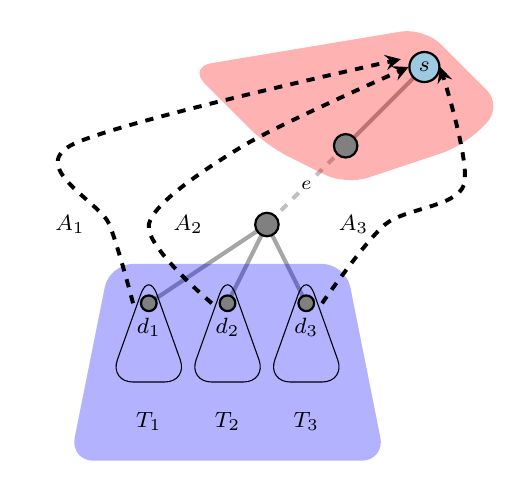
\begin{tikzpicture}
			\coordinate (s) at (1.5,2);
			\coordinate (d1) at (-2,-1);
			\coordinate (d2) at (-1,-1);
			\coordinate (d3) at (0,-1);
			\coordinate (e_upper) at (0.5,1);
			\coordinate (e_lower) at (-0.5,0);
			
			\draw [ draw=none,rounded corners = 3mm,fill=blue,fill opacity=0.3] ([shift={(-1,-2)}]d1)--([shift={(1,-2)}]d3)--([shift={(0.5,0.5)}]d3)--([shift={(-0.5,0.5)}]d1)--cycle;  
	
			\draw [ draw=none,rounded corners = 3mm,fill=red,fill opacity=0.3] ([shift={(0,0.5)}]s) --([shift={(1,-0.5)}]s)--([shift={(0.5,-1)}]s)--([shift={(0,-0.5)}]e_upper)--([shift={(-2,-1)}]s)--([shift={(-3,0)}]s)--cycle; 
	
			\node[draw,circle,fill=lightblue,thick,inner sep=2pt,minimum size=5pt] (CircleNode) at (s)  {\footnotesize $s$};
			\node[draw,circle,fill=gray,thick,inner sep=3pt,minimum size=5pt] (CircleNode) at (e_upper){};
			\node[draw,circle,fill=gray,thick,inner sep=3pt,minimum size=5pt] (CircleNode) at (e_lower){};
			\node[draw,circle,fill=gray,thick,inner sep=2pt,minimum size=5pt] (CircleNode) at (d1){};
			\node[draw,circle,fill=gray,thick,inner sep=2pt,minimum size=5pt] (CircleNode) at (d2){};
			\node[draw,circle,fill=gray,thick,inner sep=2pt,minimum size=5pt] (CircleNode) at (d3){};
	
			\Edge[style={dashed},label=$e$,fontcolor=black,color=gray!50](e_upper)(e_lower)
			\Edge[color=gray!70](s)(e_upper)
			\Edge[color=gray!70](d1)(e_lower)
			\Edge[color=gray!70](d2)(e_lower)
			\Edge[color=gray!70](d3)(e_lower)
	
			\draw [rounded corners = 3mm] ([shift={(0,0.4)}]d1)--([shift={(-0.5,-1)}]d1)--([shift={(0.5,-1)}]d1)--cycle;   
			\draw [rounded corners = 3mm] ([shift={(0,0.4)}]d2)--([shift={(-0.5,-1)}]d2)--([shift={(0.5,-1)}]d2)--cycle;
			\draw [rounded corners = 3mm] ([shift={(0,0.4)}]d3)--([shift={(-0.5,-1)}]d3)--([shift={(0.5,-1)}]d3)--cycle;
			
			\node at ([shift={(0,-0.3)}]d1){\footnotesize $d_1$};
			\node at ([shift={(0,-0.3)}]d2){\footnotesize $d_2$};
			\node at ([shift={(0,-0.3)}]d3){\footnotesize $d_3$};
			
			\node at ([shift={(-1,1)}]d1){\footnotesize $A_1$};
			\node at ([shift={(-0.5,1)}]d2){\footnotesize $A_2$};
			\node at ([shift={(0.6,1)}]d3){\footnotesize $A_3$};
	
			\node at ([shift={(0,-1.5)}]d1){\footnotesize $T_1$};
			\node at ([shift={(0,-1.5)}]d2){\footnotesize $T_2$};
			\node at ([shift={(0,-1.5)}]d3){\footnotesize $T_3$};
	
			\draw[line width=0.5mm,dashed,-stealth] plot[smooth] coordinates {([shift={(-0.2,0)}]d1)([shift={(-0.5,1)}]d1)([shift={(-1,2)}]d1)([shift={(-0.3,0.1)}]s)};
			\draw[line width=0.5mm,dashed,-stealth] plot[smooth] coordinates {([shift={(-0.2,0)}]d2)([shift={(-1,1)}]d2)([shift={(0.2,2)}]d2)([shift={(-0.2,0)}]s)};
			\draw[line width=0.5mm,dashed,-stealth] plot[smooth] coordinates {([shift={(0.2,0)}]d3)([shift={(1,1)}]d3)([shift={(2,1.5)}]d3)([shift={(0.2,0)}]s)};  
		\end{tikzpicture}
	
	\end{document}